%!TEX root = ../machine_learning.tex
% \refstepcounter{chapter}
% \part{Machine Learning}
\section*{Disclaimer and Attributions}

These are my personal notes from following Andrew Ng's Coursera Machine Learning. course. The notes contain images and text taken directly from the course. I have no copyright of the material. These notes are incomplete, and probably contain some mistakes and inaccuracies.

After finishing the first four weeks of the Coursera course, I switched to working through the complete lecture notes of Andrew Ng's Standford Machine Learning course. The lecture notes are available on the course website. They are a crucial resource for gaining good understanding of machine learning. At this point my digital note taking became minimal.

\section*{Resources}
\begin{itemize}
\item Machine Learning on Coursera: \url{https://www.coursera.org/learn/machine-learning/lecture/zcAuT/welcome-to-machine-learning}
\item Machine Learning on Standford: \url{https://github.com/afshinea/stanford-cs-229-machine-learning}
\item Standford's Intro to Probability for Computer Scientists: \url{https://web.stanford.edu/class/archive/cs/cs109/cs109.1166/}
\end{itemize}

\section{Supervised Learning}

Regression: predict real-valued output

Classification: discrete valued outputs

Training set - with $m$ number of training examples, $x$ input variables / features, $y$ outputs/targets

$(x^{(i)},y^{(i)})$ is a training example

\subsection{ Linear Regression (Uni-variable)}

Hypothesis: $h_\theta(x) = \theta_0 + \theta_1x$ 

Cost function: a function that measures the performance of the hypothesis. 
For linear regression: $\min_{\theta_0,\theta_1} \frac{1}{2m}\sum_i| h_\theta(x^{(i)})-y^{(i)} |^2 $

Squared Error Cost Function: $J = \frac{1}{2m}\sum_i( h_\theta(x^{(i)})-y^{(i)} )^2 $ 

\subsubsection{Gradient Descent for Linear Regression}

For linear regression - the least squared cost function has no local minimum

Gradient Descent will converge 

Normal Equations can be used to perform a single step solution for linear models, but GD scales better for large training sets

\subsubsection{Stochastic Gradient Descent}

Computes the gradient with respect to each training example directly and aggregates it. 

Can converge to a minimum much faster than batch gradient descent 

\subsection{Multi Variable Linear Regression}

For $n$ features, define $ x\in\mathbb{R}^{n+1}$, $0th$ indexed vector,  the features vector, where $x_0^{(i)} := 1 \forall i$  

And $\theta = (0_0,\dots,\theta_n)$  the model

The hypothesis: $h_{\theta} = \sum \theta_i x_i = \theta^T x$  

Update rule for linear regression:

$\theta_0 = \theta_0 -\alpha\frac{1}{m}\sum_i (h_\theta(x^{(i)})-y^{(i)})\cdot x_0$

and similarly for all other variables

\subsubsection{Feature Scaling}

If features are of very different dimensions, the cost function will have skewed contours in the energy landscape. The gradient descent has this ping-pong behavior.  

It helps to scale the parameters to approx. $-1 \le x_j^{(i)}\le 1$

\subsubsection{Mean Normalization}

Replace $x_i$ with $x_i - \mu_i$ to make the variable approx. 0-mean

$x_i \leftarrow \frac{x_i-\mu_i}{range}$

s = Range will be $\text{max}-\text{min}$

\subsection{Debugging Gradient Descent}

Plot the cost function when GD runs

Num of iterations depends on the algorithm / model

Automatic convergence tests:

\begin{itemize}
\item change in $J(\theta)$ decreases by less than $10^{-3}$
\end{itemize}

If the cost function value increases, try smaller $\alpha$

When visualization - either wave behavior or increase in the model

Gradient verification with FD

If $\alpha$ is small enough, GD should decrease for every iteration

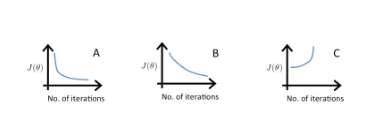
\includegraphics[width=0.9\columnwidth]{convergence.png}

A - good convergence

B - slow convergence

C - learning rate too high

Run GD with $\alpha$ with a range of values with 10-scale factor  3x from previous values

Until you find one value which is too small and one value which is too large

\subsubsection{Momentum}

\subsubsection{Netwon}

\begin{itemize}
\item no learning rate
\end{itemize}

For a function $l$ with the derivative $l^\prime(\theta)$ and second derivative, starting from an initial guess the update rule is:

$\theta := \theta - \frac{l^\prime(\theta)}{l^{\prime\prime}\theta}$

until $l^\prime(\theta)=0$. 

Newton method looks at the approximated tangent to $l(\theta)$ at the point $\theta$ and solves for where the line is equal to 0.

\subsubsection{Newton Raphson Method}

Generalization of Netwon's method to multi-variable / multi dimension settings:

$\theta = \theta - H^{-1}\nabla_\theta l(\theta)$

where $\nabla_\theta$ is a vector of partial derivatives of $l(\theta)$ with respect to $\theta$ and 

$H(\theta)=\frac{\partial^2 l(\theta)}{\partial \theta_i\partial\theta_j}$

Better and faster convergence than GD, but expensive, requires (careful) evaluation, Hessian needs to be invertible (full rank)

Fischer scoring - applying Newton's to logistic regression log likelihood function

\subsection{Polynomial Regression}

Basically, the idea here is to cheat and pre-compute the feature vector. 

For example, $(x_1 := x, x_2 := x^2, x_3 := x^3)$. 

The previous formulation and update rules hold: $\theta^Tx$

In this case it's important to scale the variables!

Other options: sqrt, cubic, squared (which might not fit a lot of models)

\subsection{Normal Equation}

For a feature vector $n$ features and $m$ data points: 

Construct a matrix $X  \in \mathbb{R}^{m\times (n+1)}$ which contains all of features for all the variables + (n+1) column which contains all 1s.

$\left( \begin{matrix} 1 & x_1^1 & ... & x_1^n \\ \vdots & x_2^1 & ... & x_2^n \\   1 & x_m^1 & ... & x_m^n \\ \end{matrix} \right)$

And collect all of the observations in a vector $y \in \mathbb{R}^m $:

And we solve for a model:

$\theta = (X^T X)^{-1} X^T y$

Now, this is true only if $X^T X$ is invertible

Feature scaling is not necessary when using the normal equation.

\subsection{GD vs. Normal Equation}

GD
\begin{itemize}
\item need to choose learning rate
\item need many iterations
\item works well when $n$ is large
\end{itemize}

Normal Equation 
\begin{itemize}
\item slow for large $n$  $O(n^3)$, $n=10k$ is where switching over could be beneficial
\item no need to choose learning rate
\item direct
\end{itemize}

\subsection{When is $X^TX$ non-invertible?}

\begin{itemize}
\item linearly dependent features - i.e. size in $m^2$ and size in feet squared
\begin{itemize}
\item remove features
\end{itemize}
\item too many features $n\ge m$ 
\begin{itemize}
  \item delete features 
  \item use regularization
\end{itemize}
\end{itemize}

\section{Classification}

\subsection{Two Class Problems}
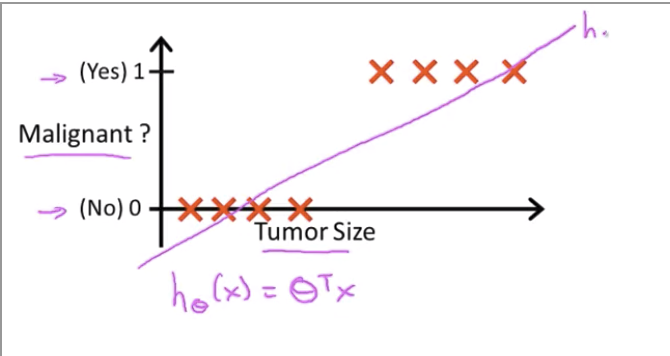
\includegraphics[width=0.9\columnwidth]{log_threshold.png}

Using linear regression model + threshold:

Classification is not actually a linear function - using linear models doesn't work well.

Labels are usually {0,1} known as negative and positive classes.

\subsubsection{Logistic Regression}

Want a model that predict a value $0\le h_\theta(x)\le 1$

Model: $h_\theta(x)=g(\theta^T x)$ 

Logistic/sigmoid function: $g(z) = \frac{1}{1+e^{-z}}$

Together: $h_\theta(x)=\frac{1}{1+e^{-\theta^T x}}$

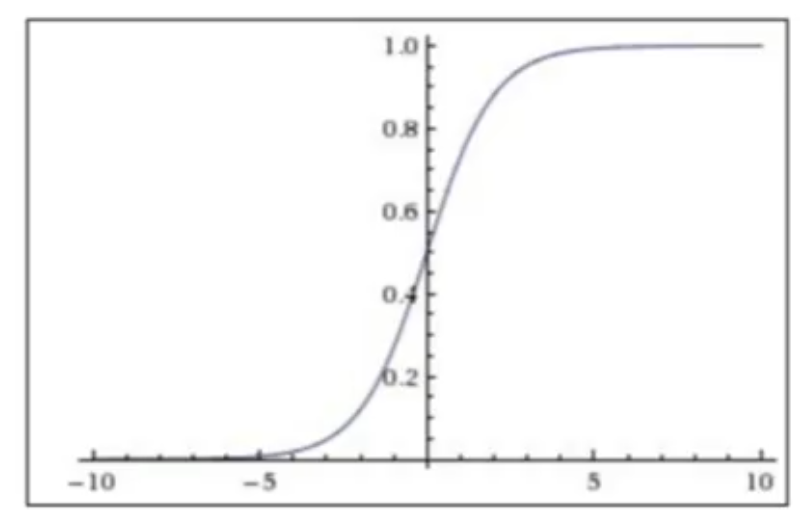
\includegraphics[width=0.9\columnwidth]{sigmoid.png}

Has  asymptotes at {0,1}

\subsubsection{Interpretation of Output}

$h_\theta(x)$ is the estimated probability that  $y=1$ on input $x$ 

$h_\theta(x) = P(y=1|x;\theta)$ 

$P(y=0|x;\theta) = 1-P(y=1|x;\theta)$

\subsubsection{Decision Boundary}

$g(z) \ge 0$.5 when $z>0$ 

$g(\theta^T x ) \ge 0.5$ when $\theta^Tx \ge 0$

(basically, here we  can derive this from $1+e^{-\theta^T x}  = 2$

The decision boundary is a function of the hypothesis and its parameters

\subsubsection{Non Linear Decision Boundaries}

Can perform a similar trick as with linear regression -> polynomial regression - build features such as $x_1^2$ etc...

So for example: 

$$\theta = \left[ \begin{matrix} -1 & 0 & 0  & 1 & 1 \end{matrix} \right]$$

$$h_\theta(x) = g(\theta^T(1,x_1,x_2,x_1^2,x_2^2 )) $$

The decision boundary will lie at $x_1^2 + x_2^2 = 1$

\subsubsection{Cost Function}

Using the linear regression cost function is non convex for the logistic regression.

$Cost(h_\theta(x),y) = \begin{cases} -\log(h_\theta(x))  ;\ \text{if} \;  y=1 \\ -\log(1-h_\theta(x))   ;\ \text{if} \;  y=0  \end{cases}$

This formulation has desirable properties: 

$(h(x)=0, y = 0)$ or$(h(x) = 1, y = 1)$  - cost = 0

Very high penalization if $(h(x)=1, y = 0)$ or$(h(x) = 0, y = 1)$ due to the cost function going asymptotically to $\infty$ :

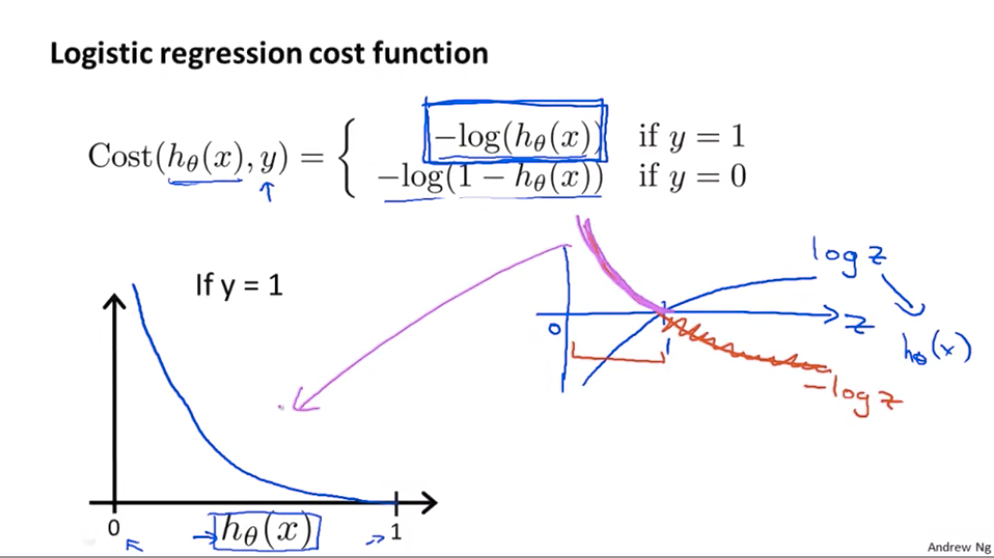
\includegraphics[width=0.8\columnwidth]{cost_function.png}

\subsubsection{Simplified Cost Function}

A generalized cost function is: 

$Cost(h_\theta (x), y) =-y\log(h_\theta(x))-(1-y)\log(1-h_\theta(x))  $

And summarizing over all examples:

$J(\theta)= -\frac{1}{m} \sum_{i=1}^{m} y^{(i)}\log(h_\theta(x^{(i)}))+(1-y^{(i)})\log(1-h_\theta(x^{(i)}))$

To minimize, solve for parameters:

$\min_{\theta} J(\theta) $ 

Output / new prediction: $h_\theta(x) = \frac{1}{1+e^{-\theta^T x}}$

$\frac{\partial}{\partial_{\theta_j}} J(\theta) = \frac 1 m \sum_i (h_\theta(x^{(i)})-y^{(i)})x_j^{(i)}$

Exactly the same update as linear regression. Here the main difference is that $h_\theta$  went from $\theta^T x $ to $\frac{1}{1+e^{-\theta^Tx}}$

And the update rules are:

$\theta_j := \theta_j - \frac{\alpha}{m} \sum_{i=1}^m (h_\theta(x^{(i)}) - y^{(i)}) x_j^{(i)}$

And vectorized:

$\theta:=\theta - \frac{\alpha}{m}X^T(g(X\theta)-\vec{y})$

\subsection{ Maximum Likelihood Estimation + Convexity}

Convexity: gives us lower bounds on the first order approximation of the function (i.e. the first order approximation is guaranteed to be larger than or equal to the real function value).

Assuming that the target variables and input are related via the equation: 

$y^{(i)}=\theta^Tx^{(i)}+\epsilon^{(i)}$

where $\epsilon$ are IID (independently and identically distributed) error terms the captures unmodeled effects, i.e random noise.

Assuming $e^{i}\sim\mathcal{N}(0,\sigma^2)=\frac{1}{\sqrt{2\pi}\sigma}\exp\left(-\frac{(\epsilon^{(i)})^2}{2\sigma^2}\right)$

That implies that: $p(y^{(i)}|x^{(i)};\theta)=\frac{1}{\sqrt{2\pi}\sigma}\exp\left(-\frac{(y^{i}- \theta^Tx^{(i)})^2}{2\sigma^2}\right)$ - this does not depend on $\theta$, the model is not a random variable! 

For the entire model's training set $X$  we can define this the likelihood function of the model : $L(\theta)=L(\theta;X;\vec{y})=p(\vec{y}|X;\theta)$

$L(\theta) = L(\theta;X,\vec y) = p(\vec y| X;\theta)$

Since all of the observations are independent:

$L(\theta)= \Pi_{i} p(y^{(i)}| x^{(i)};\theta) = \Pi_{i} \frac{1}{\sqrt{2\pi}\sigma}\exp\left(-\frac{(y^{i}- \theta^Tx^{(i)})^2}{2\sigma^2}\right) $

Maximum likelihood: we should choose a model $\theta$ so as maximize the probability of the data: $\theta$ should maximize $L(\theta)$. 

By deriving the function that maximizes $\log L(\theta)$ , product becomes a series sum and we simply need to maximize the $\frac 1 2 \sum_i (y^{(i)}-\theta^T x^{(i)})^2$ which is the original least-squares cost function.

Note that this does not depend on $\sigma$ !

\subsubsection{Maximum A Posteriori}

\yeara{TODO}

\subsection{Locally Weighted Linear Models}

\subsection{Optimization Techniques}

There following algorithms are alternatives to GD that do not require choosing a learning rate:

\begin{itemize}
\item Conjugate Gradient
\item BFGS
\item L-BFGS
\end{itemize}

Advantages:
\begin{itemize}
\item No learning rate
\item Faster than GD
\item Line search
\end{itemize}

Disadvantages
\begin{itemize}
\item More complex
\item Prob. don't imp. yourself
\end{itemize}

\subsubsection{Multi-Class Classification Problems}

\subsubsection{One vs. All}

For example: tagging emails according to multiple classes; weather (rainy, sunny)

For each class, train a logistic regression classifier $h_{\theta}^{(i)}(x)$ that predicts that probability that $y=i$.

For new input choose $\max_ih_\theta^i(x)$

\section{ML Algorithm Design and Debugging}

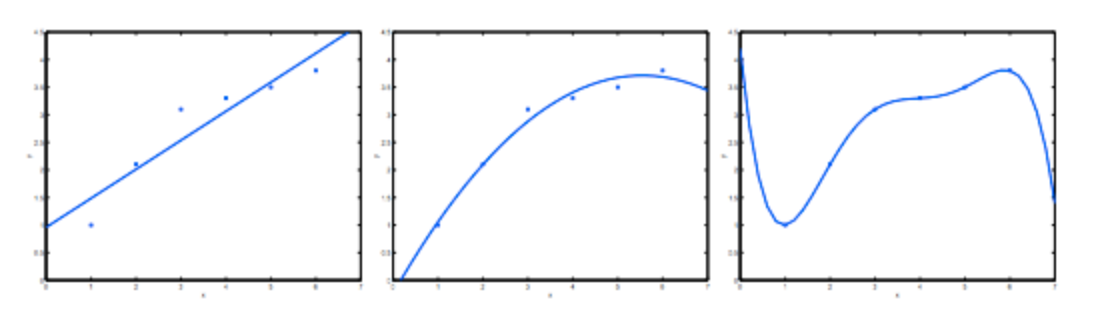
\includegraphics[width=0.5\columnwidth]{overfitting.png}

Underfitting $\rightarrow$ high bias.

Overfitting $\rightarrow$  high variance

High variance - fitting a high order polynomial can be used to fit almost any function, not enough data to give a good hypothesis

If we have too many features, the learned hypothesis may fit the training data very well, but fail to generalize

\subsection{Model Selection and Train/Validation/Test Sets}
Just because a learning algorithm fits a training set well, that does not mean it is a good hypothesis. It could over fit and as a result your predictions on the test set would be poor. The error of your hypothesis as measured on the data set with which you trained the parameters will be lower than the error on any other data set.

Given many models with different polynomial degrees, we can use a systematic approach to identify the 'best' function. In order to choose the model of your hypothesis, you can test each degree of polynomial and look at the error result.

One way to break down our dataset into the three sets is:

Training set: 60

Cross validation set: 20

Test set: 20

We can now calculate three separate error values for the three different sets using the following method:

Optimize the parameters in $\theta$ using the training set for each polynomial degree.
Find the polynomial degree d with the least error using the cross validation set.
Estimate the generalization error using the test set with $J_{test}(\theta(d))$, ($d = \theta$ from polynomial with lower error). 
This way, the degree of the polynomial d has not been trained using the test set.

\subsection{Regularization}

Penalizing the $\theta$ too much leads to high bias in the model, i.e. strong underfitting. 

When adding regularization, the error should be computed without the regularization term - i.e. now the error function and the cost function are different.


How to choose regularization weight:
\begin{itemize}
\item Create a list of lambdas (i.e. $\lambda \in {0,0.01,0.1, 1, 10, 100}$);
\item Create a set of models with different degrees or any other variants.
\item Iterate through the $\lambda$s and for each $\lambda$ go through all the models to learn some $\theta$.
\item Compute the cross validation error using the learned $\theta$ (computed with $\lambda$) on the $J_{CV}(\theta)$ without regularization.
\item Select the best combo that produces the lowest error on the cross validation set.
\item Using the best combo $\theta,\lambda$ apply it to the test set to see if it generalizes.
\end{itemize}

\subsubsection{Addressing Overfitting}

Reduce number of features

Requires deciding which feature to keep and discard
Model selection algorithms

Regularization

\begin{itemize}
\item keep features but reduce magnitude / values of $\theta_j$ 
\item works well when there are a lot features, each of which contributes less
\end{itemize}

Modify the cost function by penalizing the parameters:

Penalize higher order parameters: equiv to reducing the model to lower order model - simplfying the model

Penalize all parameters  - trying to keep the hypothesis small, usually corresponds to smoother functions

So now the objective has a data term and a regularization term.

The regularization term: $\lambda\sum_{j=1} \theta_j^2 $ keeps all of them small

If $\lambda $ is very large, in linear reg., all model parameters will be close to 0 and $h_\theta(x) = \theta_0$ 

\subsection{Polynomial Degree and Bias vs. Overfitting}

The relationship between the degree of the polynomial $d$ and the underfitting or overfitting of our hypothesis.

We need to distinguish whether bias or variance is the problem contributing to bad predictions. 
High bias is underfitting and high variance is overfitting. Ideally, we need to find a golden mean between these two.
The \emph{training} error will tend to decrease as we increase the degree $d$ of the polynomial.

At the same time, the \emph{cross validation error} will tend to decrease as we increase d up to a point, and then it will increase as d is increased, forming a convex curve.

High bias (underfitting): both $J_{train}(\theta)$ and $J_{CV}(\theta)$ will be high. Also, $J_{CV}(\theta)\approx J_{train}(\theta)$.

High variance (overfitting): $J_{train}(\theta)$ will be low and $J_{CV}(\theta)$ will be much greater than $J_{train}(\theta)$.

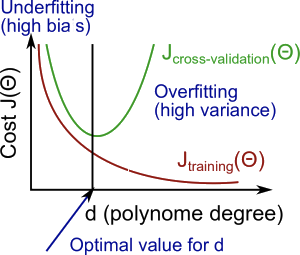
\includegraphics[width=0.9\columnwidth]{bias_variance.png}

\subsection{Learning Curve}

With a smaller number of training examples, the error cost on the training set or cross validation set should remain relatively low. As the number of training examples grows, the error will increase (but approximately asymptotically), as it become harder to fit all examples perfectly. At the same time, the cross-validation error should decrease.

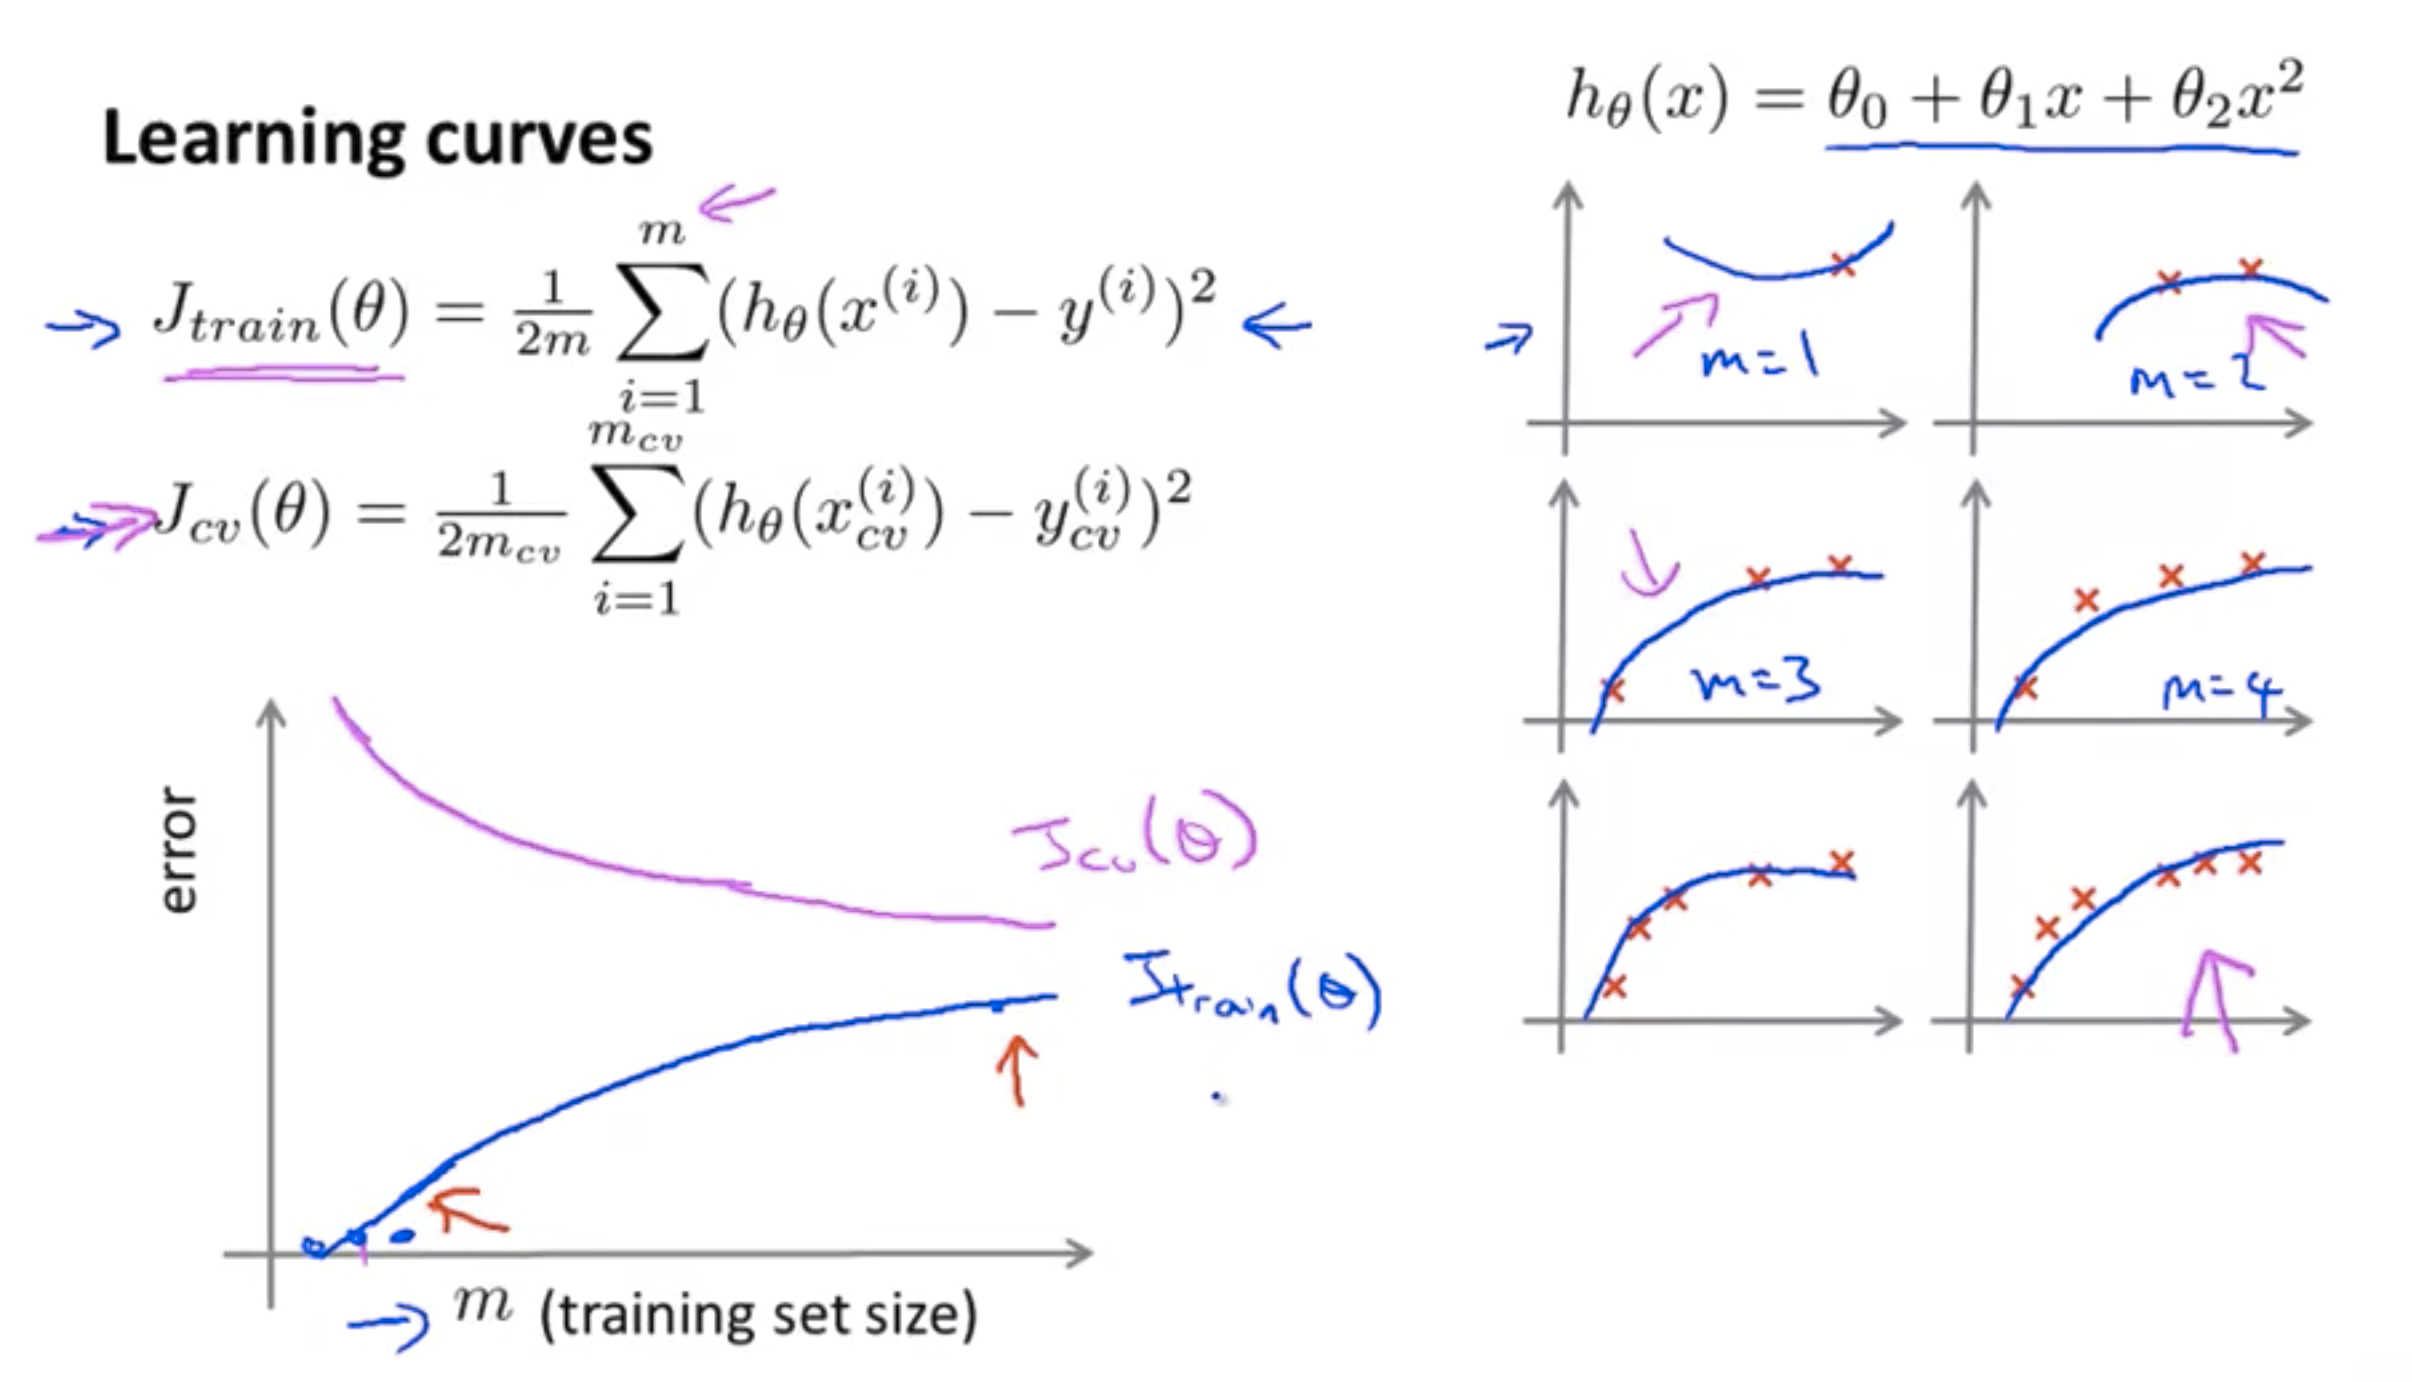
\includegraphics[width=0.9\columnwidth]{learning_curve.png}

\subsubsection{High Bias Case}

In this case the model does not have enough degrees of freedom to fit the data. Adding more data points will not help the performance of the model. 

One will observe that the cross validation error will decrease initially, and then stagnate. 
The training error will increase until it comes close to the cross-validation error.
Both of these errors will be high.

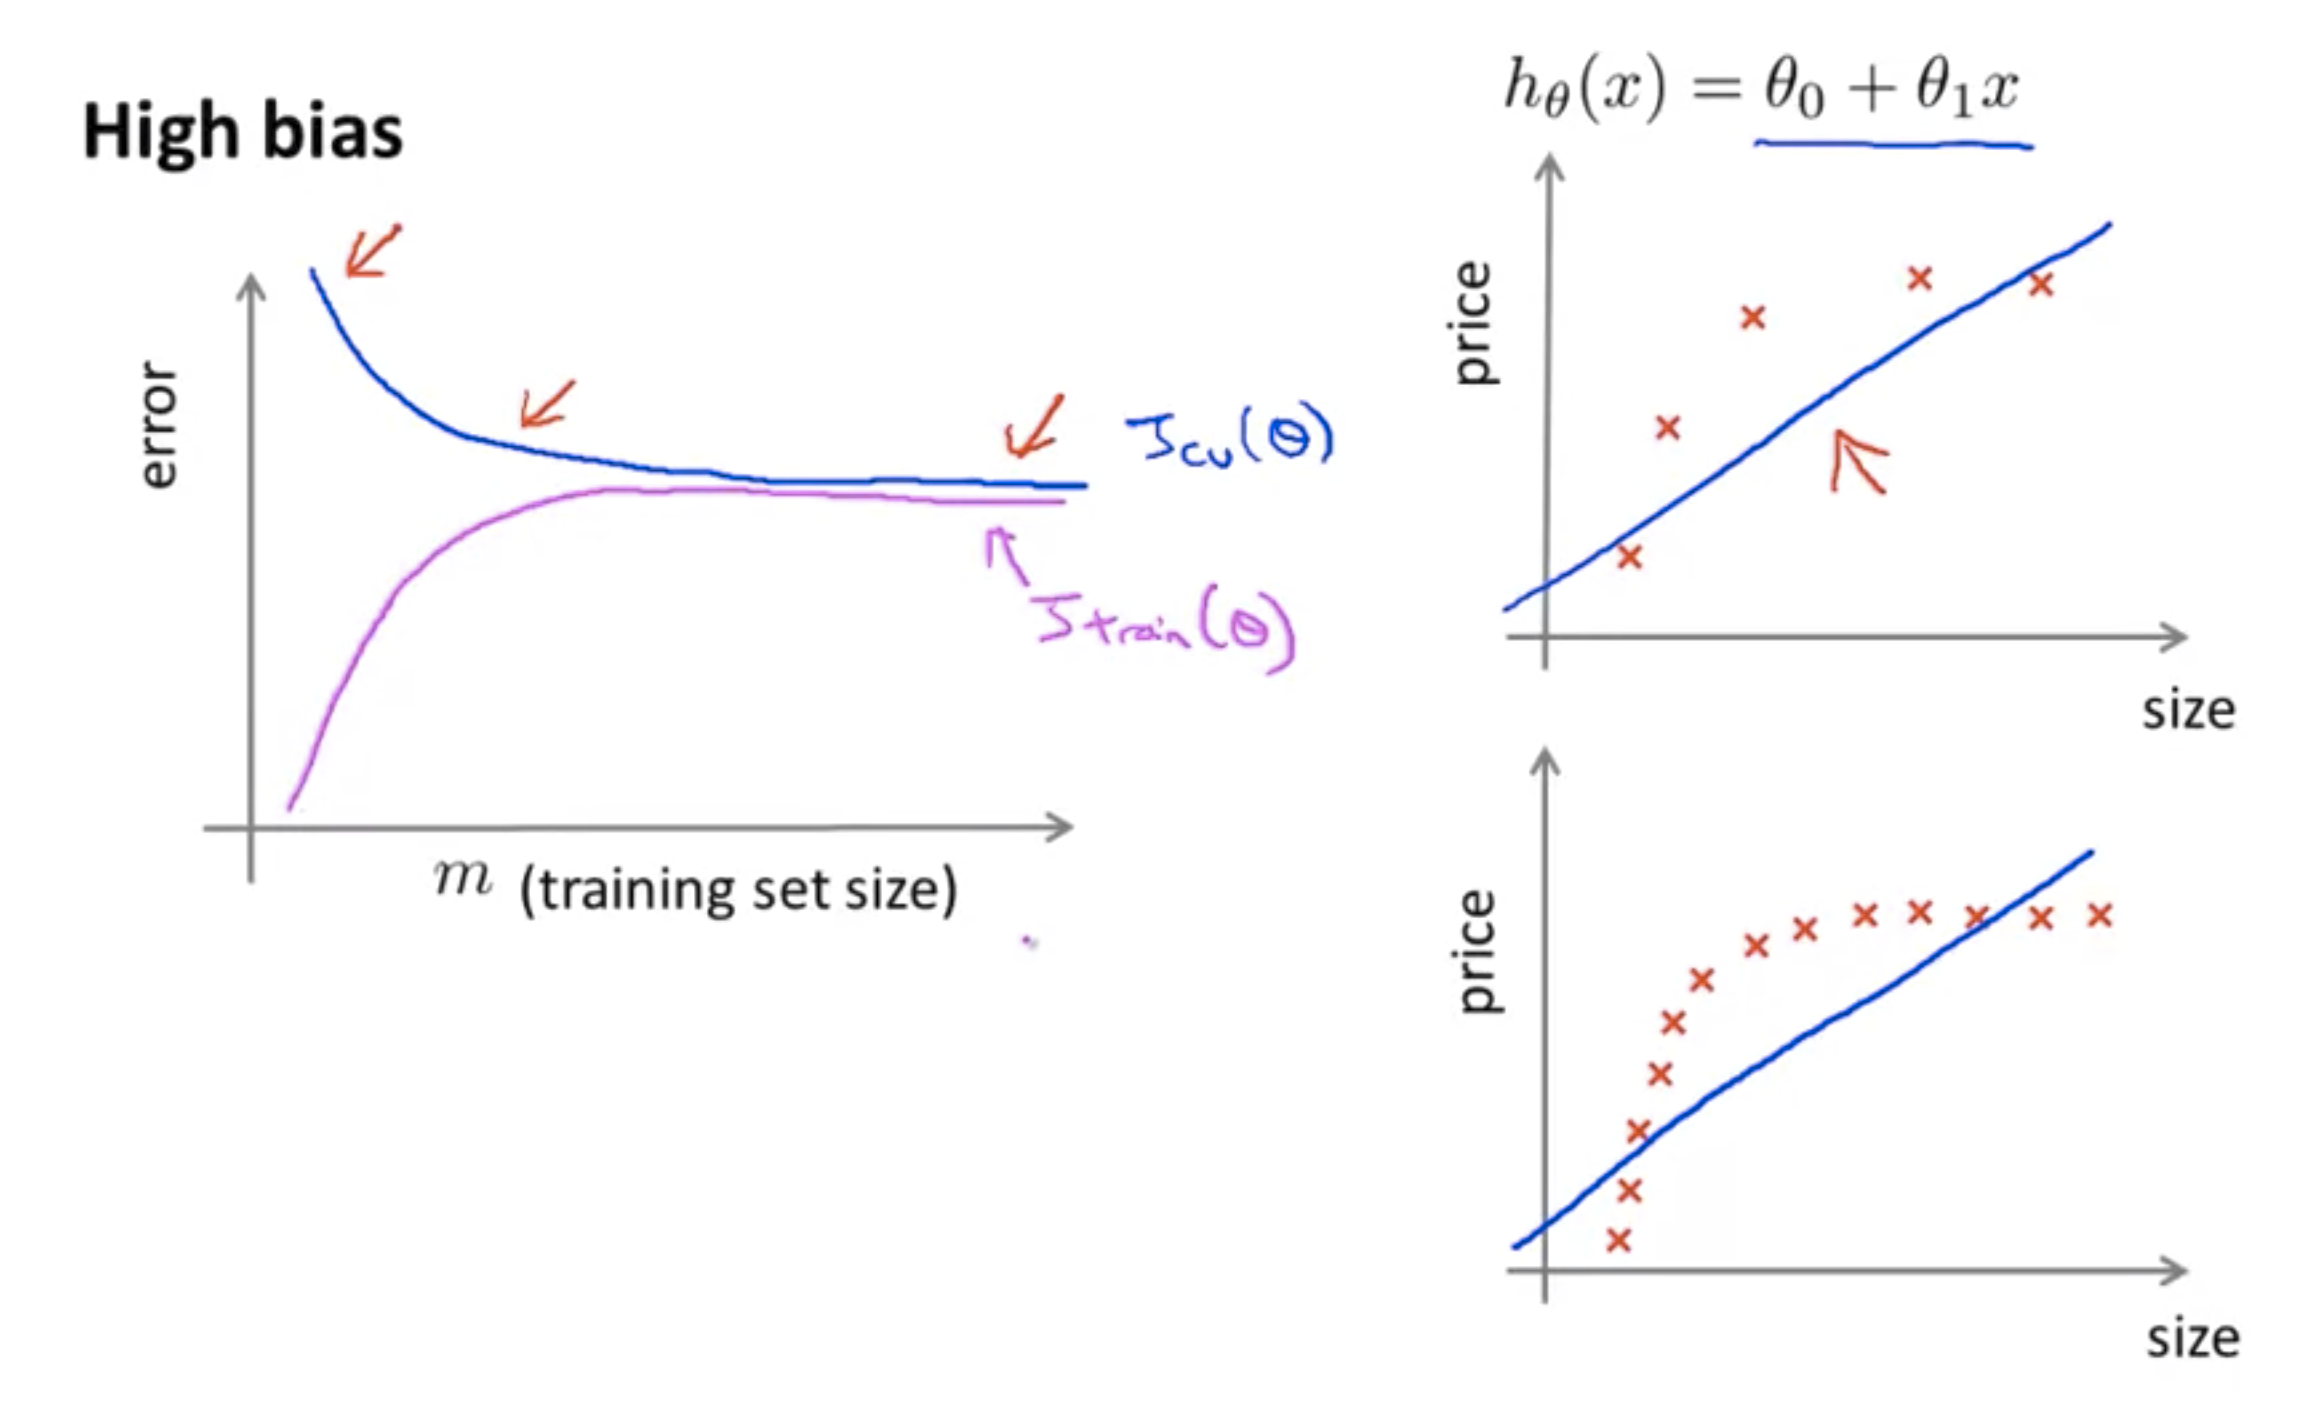
\includegraphics[width=0.9\columnwidth]{learning_curve_bias.png} 

\subsubsection{High Variance Case}

The training error will remain low, although increase slightly as it becomes harder and harder to fit more training examples.

The cross validation error will remain high, maybe will decrease.

We will observe a large gap between the training error and the cross validation error. In the high variance case, adding more training examples can help.

\subsection{Evaluating a Hypothesis}

Regression error = (normalized) $(h_\theta(x^(i)) - y^{(i)})^2$

Misclassification error = (normalized) $\sum err (h_\theta(x^{(i)}), y^{(i)})$

Trouble shooting options:

Getting more training examples $\rightarrow$ fixes high variance.
Trying smaller sets of features $\rightarrow$ fixes high variance.
Trying additional features - solution for high bias
Trying polynomial features - solution for high bias
Increasing $\lambda$ - quick and easy - fixes high bias
decreasing $\lambda$ - fixes high variance

\subsubsection{Neural Networks and Overfitting}

Smaller networks - fewer parameters, more prone to underfitting - computationally cheaper
Larger networks - more parameters, prone to overfitting - expensive, use regularization. 
Usually larger network + regularization results in better performance.


\subsection{Approaching ML Problems}

Start with simple models and iterate quickly. 
Implement a quick and dirty algorithm to quickly identify error and hard examples.
It is very hard to decide in advance what would be a good model.

Structure your data into train, validation and test tests. 

Systematically test and plot the model performance (learning curve, error rates) with the variation of the model hyperparameters. 
Doing this avoids premature optimization. Use data and evidence to decide where to spend our time. 

Error analysis - manually examine the model's errors. Try to spot any patterns or features that can be used to classify them correctly. 


\subsubsection{Numerical Evaluation}

It is best if it's a single number. 

Example: does stemming help model performance for spam filtering? 
In that case, error analysis might not be that useful for understand if stemming works, and it is easier to try it and evaluate the performance.

The cross validation error is a natural choice for such a number.

\subsection{Error Classes for Skewed Classes}

Example: cancer classification.
Performance: 1\% error 99\% accuracy on the test set.

But only 0.5\% of the patients have cancer. In this case, predicting no one has cancer gives 99.5\% accuracy.

\subsubsection{Precision-Recall}

True positive
True negative
Type 1 Error - False positive - Predict an event when there was no event
Type 2 Error - False negative - Predict no event when in fact there was an event.


$\text{Precision} = \frac{\text{true positive}}{\text{\# predicted positive}} = \frac{\text{true positive}}{\text{true pos + false pos}}$

$\text{Recall} = \frac{\text{true positive}}{\text{actual positive}} = 
\frac{\text{true positive}}{\text{true pos + false neg}} $

In case of a model that predict 0 for everything (for example), the recall = 0. 

Precision-Recall curves summarize the trade-off between the true positive rate and the positive predictive value for a predictive model using different probability thresholds.

They are appropriate for imbalanced datasets.

In the case of logistic regression, we can set the trade off between precision and recall by adjusting the decision boundary. For example, setting a high decision boundary towards the underrepresented class (for example, in that case, actual cancer) will increase precision but lower recall. 

Setting the decision boundary to be lower - i.e. - labeling anyone with more than 30\% of cancer as cancer will increase the recall but lower the precision.

\subsubsection{ROC -  Receiver Operating Characteristic curve}

Summarize the trade-off between the true positive rate and false positive rate for a predictive model using different probability thresholds.

ROC curves are appropriate when the observations are balanced between each class

Convolution is a mathematical operation on two functions that produces a third function expressing how the shape of one is modified by the other.

$(f\star g)(t) = \int_{-\infty}^{\infty} f(\tau)\cdot g(t-\tau)d\tau = \int_{-\infty}^{\infty} f(t-\tau)\cdot g(\tau)d\tau $

Commutative. 

For functions which only have limited support the integration is only done on the valid domain.

\subsection{L1 vs L2 Norm}

L2 norm strongly penalizes outliers. For good data with some very far outlier it might not generate the "best" fit as judged by a human observer.

L1 favors sparse coefficients.


\section{Unsupervised Learning}

Algorithms for finding structure in data.

\section{Clustering}

The clustering problem: given an unlabeled data set, group the data into coherent  subsets or into coherent clusters for us.

\subsection{K Means}

\begin{itemize}
\item $K$ number of clusters + initialization
\item Training set ${x^{(1)},x^{(2)}\dots,x^{(m)}}$
\item $x\in\mathbb{R}^n$
\item By convention, drop $x_0=1$
\end{itemize}

Randomly initialize K cluster centers
While not converged:
1. iterate over data and assign a cluster for each data point based on distance to center
2. re-compute the cluster mean

If a cluster becomes empty - remove the cluster

Or randomly re-initialize the cluster

\subsubsection{K Means for Non Separated Clusters}

\subsubsection{K Means Cost Function}

Assuming: 

$c^{(i)}$ index of cluster to which the example $x^{(i)}$ belongs to.

$\mu_k \in \mathbb R ^n $ cluster centroid 

$\mu_{c^{(i)}} \in \mathbb R ^n $ location of the cluster centroid to which example $x^{(i)}$ has been assigned

Example cost for point $Cost(x^{(i)}) = \|x^{(i)} - \mu_{c^{(i)}} \|^2$ 

$J(c^{(1)},\dots, c^{(k)})= \frac{1}{m}\sum_i \|x^{(i)} - \mu_{c^{(i)}} \|^2 $

The objective is to minimize the cost function *distortion* with respect to the clusters (both labelling and centers).

So what k-means algorithm is actually doing is:

1. minimize the cost function with respect to cluster assignments $c^{(i)}$

2. minimize the cost function with respect to cluster centroids $\mu_k$ 

(so basically block coordinate descent?)

\subsubsection{Random Initialization}

\begin{itemize}
\item $K < m$
\item Randomly pick $K$ training examples and set the cluster means to these examples
\end{itemize}

K-mean can get stuck in a local optima - to avoid this a good option is to run k-mean multiple times and get as good global optimum

For multiple initializations - run K-means loads of times, pick the clustering which results in the lowest cost function

This works well for small $K < 10$ .

For large $K$s it is not as effective.

\subsubsection{Number of Clusters - Elbow Method}

Choosing the right K 

Plot the cost function with respect to the number of clusters:

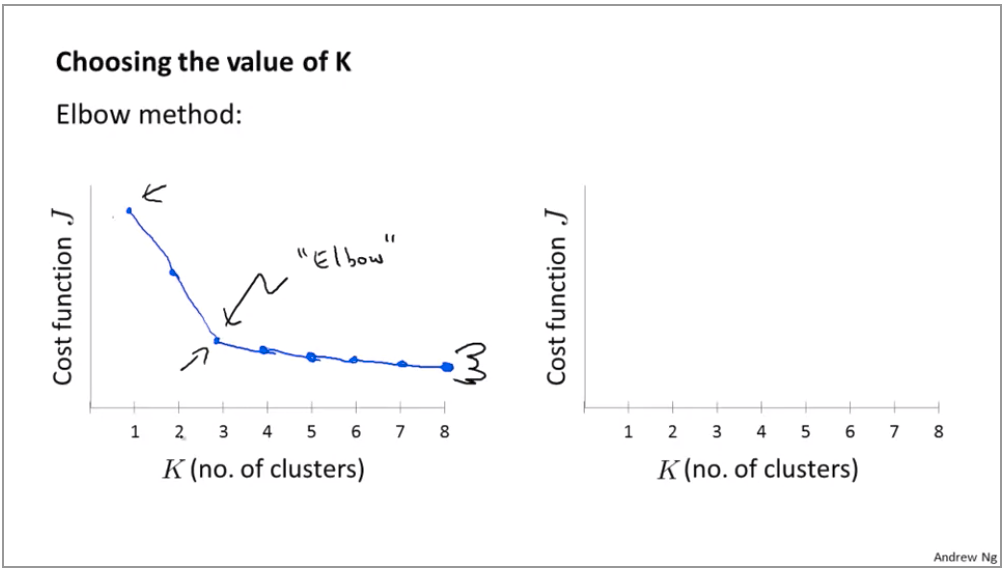
\includegraphics[width=0.9\columnwidth]{elbow.png}

In practice it is usually a bit harder, and it is not clear that there is such a transition where the distortion stops.

\subsection{Gaussian Mixture Models and Expectation Maximization}

Refer to Standford Course. 

Main idea: soft, probabilistic K-Means.

\section{Dimensionality Reduction}

\subsection{PCA}

PCA is trying to find a lower dimension representation of that data which minimizes the squared distance error of the data from the representation.

Before PCA it is standard practice to perform mean normalization and feature scaling. 

\subsubsection{PCA vs Linear Regression}

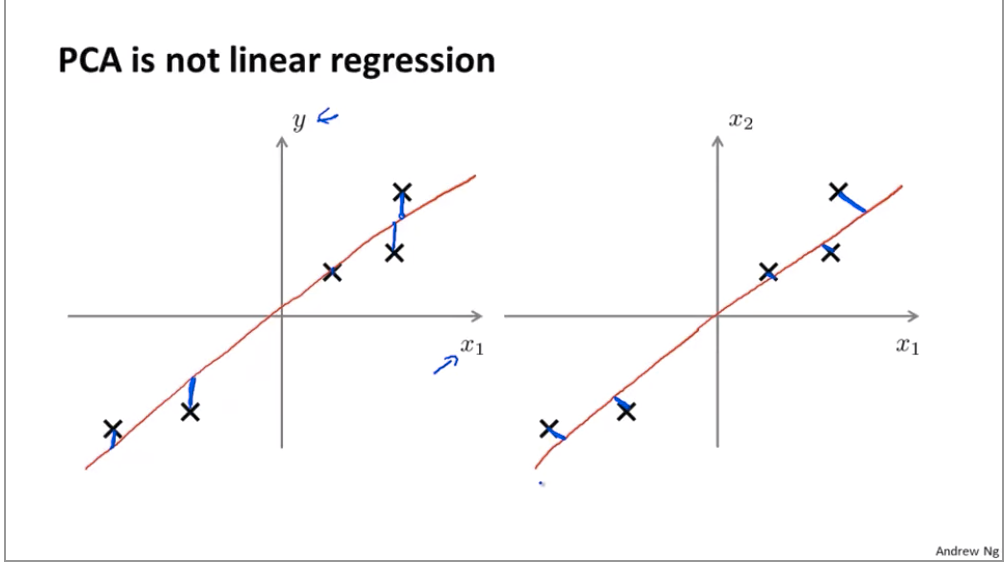
\includegraphics[width=0.9\columnwidth]{PCA_Linear.png}

We do not treat $y$ as a special variable

Minimized projected error vs. minimize distance from line


\section{Decision Trees}
Recursive repartition of the data. 

\subsection{Random Forest Regression}

An ensemble of decision trees. During learning tree nodes are split using random variable subset of data features.

All trees vote to produce final result.

For best results trees should be as independent as possible. Splitting using a random subset of features achieves this.

Averaging the product of the trees reduces overfitting to noise

5-100 Trees.

\subsection{Random Fern Regressors}

\section{RANSAC}

A method for dealing with noisy data. 

Partition the method 

Is not determinant, depends on the subset selection, and is not guaranteed to converge.

\begin{enumerate}
\item Select a random subset of the original data. Call this subset the hypothetical inliers.
\item A model is fitted to the set of hypothetical inliers.
\item All other data are then tested against the fitted model. Those points that fit the estimated model well, according to some model-specific loss function, are considered as part of the consensus set.
\item The estimated model is reasonably good if sufficiently many points have been classified as part of the consensus set.
\item Afterwards, the model may be improved by reestimating it using all members of the consensus set.
\end{enumerate}

```
Given:
    data – a set of observations
    model – a model to explain observed data points
    n – minimum number of data points required to estimate model parameters
    k – maximum number of iterations allowed in the algorithm
    t – threshold value to determine data points that are fit well by model 
    d – number of close data points required to assert that a model fits well to data

Return:
    bestFit – model parameters which best fit the data (or nul if no good model is found)

iterations = 0
bestFit = nul
bestErr = something really large
while iterations < k {
    maybeInliers = n randomly selected values from data
    maybeModel = model parameters fitted to maybeInliers
    alsoInliers = empty set
    for every point in data not in maybeInliers {
        if point fits maybeModel with an error smaller than t
             add point to alsoInliers
    }
    if the number of elements in alsoInliers is > d {
        % this implies that we may have found a good model
        % now test how good it is
        betterModel = model parameters fitted to all points in maybeInliers and alsoInliers
        thisErr = a measure of how well betterModel fits these points
        if thisErr < bestErr {
            bestFit = betterModel
            bestErr = thisErr
        }
    }
    increment iterations
}
return bestFit
```

\section{ML Algorithm Design}

General process of building a ML product:

\begin{enumerate}
\item What is the objective? prediction, recommendation, clustering, search, etc.
\item Pick the right algorithm: supervised vs unsupervised, classification vs regression, generalized linear model / decision tree / neural network / etc.
\item Pick / engineer relevant features based on available data.
\item Pick metrics for model performance.
\item Optionally, comment on how to optimize the model for production.
\end{enumerate}

\section{Other Important Topics}

This topics were out of scope of this document, I worked with the Stanford Machine Learning lecture notes.

\subsection{Generative Models}

\subsection{Support Vector Machines}

\subsection{Boosting}
Collaborative filtering.

Learning strong classifiers from weak classifiers.

\subsection{Naive Bayes Classifier}

% \section{Neural Networks}
% http://karpathy.github.io/neuralnets/

